% 
% File naaclhlt2015.tex
%


\documentclass[11pt,letterpaper]{article}
\usepackage{naaclhlt2015}
\usepackage{times}
\usepackage{latexsym}
\usepackage{amsmath}
\usepackage{amssymb}
\usepackage{etex}
\usepackage{booktabs}
\usepackage{tikz}
\usepackage{multirow}


\usepackage{tikz-qtree}
\usepackage{tikz-dependency}
\usepackage{proof}
\usepackage{fullpage}
\usepackage{todonotes}
\usepackage{multicol}
\usepackage{url}

\newtheorem{theorem}{Theorem}[section]
\newtheorem{lemma}[theorem]{Lemma}
\newtheorem{proposition}[theorem]{Proposition}
\newtheorem{corollary}[theorem]{Corollary}

\newenvironment{proof}[1][Proof]{\begin{trivlist}
\item[\hskip \labelsep {\bfseries #1}]}{\end{trivlist}}
\newenvironment{definition}[1][Definition]{\begin{trivlist}
\item[\hskip \labelsep {\bfseries #1}]}{\end{trivlist}}
\newenvironment{example}[1][Example]{\begin{trivlist}
\item[\hskip \labelsep {\bfseries #1}]}{\end{trivlist}}
\newenvironment{remark}[1][Remark]{\begin{trivlist}
\item[\hskip \labelsep {\bfseries #1}]}{\end{trivlist}}

\newcommand{\qed}{\nobreak \ifvmode \relax \else
      \ifdim\lastskip<1.5em \hskip-\lastskip
      \hskip1.5em plus0em minus0.5em \fi \nobreak
      \vrule height0.75em width0.5em depth0.25em\fi}

\usepackage[font=footnotesize]{caption}
\usepackage{amsfonts}
\usepackage{amsmath}
\usepackage{xspace}
\DeclareMathOperator*{\argmax}{arg\,max}
\DeclareMathOperator*{\argmin}{arg\,min}

\usepackage{algpseudocode}
\usepackage{algorithm}

\usetikzlibrary{arrows}
\usetikzlibrary{decorations.markings}
\tikzset{
  >=latex,text height=1.5ex,text depth=0.25ex
}

\newcommand{\nonterms}{\mathcal{N}}
\newcommand{\END}{\mathrm{END}}
\newcommand{\START}{\mathrm{START}}
\newcommand{\rules}{\mathcal{G}}
\newcommand{\terms}{\mathcal{T}}
\newcommand{\LeftS}{\mathcal{L} }
\newcommand{\RightS}{\mathcal{R} }

\newcommand{\Left}[1]{#1_{\Leftarrow}}
\newcommand{\Right}[1]{#1_{\Rightarrow}}
\newcommand{\Span}[1]{\langle #1 \rangle}
\newcommand{\tri}{\langle \Left{m}, \Right{m} \rangle}

\newcommand{\Tag}[1]{\texttt{#1}}
\newcommand{\Root}{r}

\newcommand{\RuleSym}{\mathrm{rule}}
\newcommand{\Rule}[3]{#1 \rightarrow #2\ #3}
\newcommand{\RuleA}[3]{#1 \rightarrow #2^*\ #3}
\newcommand{\RuleB}[3]{#1 \rightarrow #2\ #3^*}
\newcommand{\BinFN}[1]{\mathrm{bin}({#1})}
\newcommand{\TagFN}[1]{\mathrm{tag}({#1})}
\newcommand{\WordFN}[1]{x_{#1}}
\newcommand{\Reals}{\mathbb{R}}
\newcommand{\Head}{\mathrm{head}}
\newcommand{\ParseName}{\textsc{Pad}\xspace}
%\newcommand{\ParserUrl}{\url{https://github.com/srush/PhraseDep}}
\newcommand{\ParserUrl}{\url{https://github.com/ikekonglp/Converter}}

\newcommand{\smrcomment}[1]{\textcolor{green}{\bf \small [#1 --smr]}}
\newcommand{\lpkcomment}[1]{\textcolor{red}{\bf \small [#1 --lpk]}}
\newcommand{\nascomment}[1]{\textcolor{blue}{\bf \small [#1 --nas]}}


\setlength\titlebox{5.5cm}    % Expanding the titlebox

\title{Transforming Dependencies into Phrase Structures }


% \author{Lingpeng Kong \quad Alexander M.~Rush \quad Noah A.~Smith}
\author{Lingpeng Kong\\
      School of Computer Science\\
  	Carnegie Mellon University\\
  	Pittsburgh, PA, USA\\
  {\tt lingpenk@cs.cmu.edu}
	  \And
      Alexander M.~Rush\\
	    Facebook AI Research \\
	    New York, NY, USA \\
	    {\tt srush@seas.harvard.edu}
	  \And
	Noah A.~Smith\\
      School of Computer Science\\
  	Carnegie Mellon University\\
  	Pittsburgh, PA, USA\\
  {\tt nasmith@cs.cmu.edu}}


%% For drawing the traps/tris.

\date{}

\begin{document}
\maketitle
\begin{abstract}
We present a new algorithm for transforming dependency parse trees into
phrase-structure parse trees.  We cast the problem as  structured
prediction and learn a statistical model.  Our algorithm is faster than traditional
phrase-structure parsing and achieves 90.4\% English parsing accuracy and 82.4\% Chinese parsing accuracy, near to the state of
the art on both benchmarks.

  % Motivated by the increase in accuracy of statistical dependency
  % parsers, we consider the problem of decoding phrase-structure parses
  % directly from predicted dependency trees. Unlike past rule-based
  % approaches, we treat this as a structured prediction problem using a
  % specialized context-free parser. Since our parser makes use of the
  % predicted dependency structure it is asymptotically faster and much
  % simpler than a standard lexicalized parser. However, despite its
  % simplicity, it still yields high-accuracy phrase-structure parses on
  % experiments in both English and Chinese.



\end{abstract}

\section{Introduction}


Natural language parsers typically produce phrase-structure (constituent) trees or dependency trees.  These representations capture
some of the same syntactic phenomena, and the two can be produced
jointly \cite{klein2002fast,hall2008dependency,carreras2008tag,rush2010dual}.  Yet it
appears to be completely unpredictable which will be preferred by a
particular subcommunity or used in a particular application.  Both continue to receive the attention of
parsing researchers.


Further, it appears to be a historical accident that phrase-structure
syntax was used in annotating the Penn Treebank, and that English
dependency annotations are largely derived through mechanical,
rule-based transformations (reviewed in Section~\ref{sec:background}).  Indeed,
despite extensive work on direct-to-dependency parsing algorithms
(which we call \emph{d-parsing}), the most accurate dependency
parsers for English still involve phrase-structure parsing (which we
call \emph{c-parsing}) followed by rule-based extraction of
dependencies \cite{kong2014empirical}.
 % \nascomment{could reference the table here, or
 %  just cite}.

What if dependency annotations had come first?  Because d-parsers are
generally much faster than c-parsers, we consider an alternate
pipeline (Section~\ref{sec:pardeps}): d-parse first, then transform the dependency representation
into a phrase-structure tree constrained to be consistent with the
dependency parse.  This idea was explored by  \newcite{xia2001converting} and
\newcite{xia2009towards} using hand-written rules.  Instead, we present a data-driven
algorithm using the structured prediction framework (Section~\ref{sec:strpred}).  The approach can be
understood as a specially-trained coarse-to-fine
decoding algorithm where a d-parser provides ``coarse'' structure and
the second stage refines it \cite{charniak2005coarse,petrov2007improved}.

Our lexicalized phrase-structure parser, \ParseName, is asymptotically faster than
parsing with a lexicalized context-free grammar: $O(n^2)$ plus
d-parsing, vs.~$O(n^5)$ worst case runtime in sentence length $n$,
with the same grammar constant.  Experiments show
that our approach achieves linear observable
runtime, and accuracy similar to
state-of-the-art phrase-structure parsers without reranking or
semi-supervised training (Section~\ref{sec:exper}).





% There are two main grammatical
% frameworks used for statistical syntactic prediction: phrase-structure parsers and
% dependency parsers \cite{}. The two offer a
% trade-off: phrase-structure parsing is very accurate \lpkcomment{i am not sure if the accurate is the right word here... dep parser is also very accuarate.} and provides a
% full context-free syntactic representation; dependency parsing is
% often faster, but still
% predicts much of the useful\lpkcomment{again... here i think maybe we should say different rather than imply which is more useful?} syntactic structure.

% We can quantify this difference by looking
% at the dependency prediction accuracy of phrase-structure parsers. Table~\ref{fig:depcomp} shows this comparison across several widely-used parsers. Note that the best models are phrase-structure parsers, but that recent advances in dependency parsing have led to comparably high-accuracy dependency parsers.\lpkcomment{this is a little confusing? there are two ways to get dependencies, c-parsing and d-parsing, but here it seems we are comparing the acc between phrase-structure and dependency parsing acc? they are two different systems....}

% The natural reverse question is how well do these dependency parsers perform at phrase-structure prediction? Is it reasonable to use dependency parsers for tasks that require phrase-structure trees as input? \lpkcomment{i would like to put the benefits of doing this dep2phrase thing in the intro maybe? 1) it is very fast since dep prunes away a lot not useful cky chart item 2) dep can server as features in this problem, so that we can aim at higher acc with easy cky model. (actually, i believe the dep parsers can see syntactical information which is not easy to see when using cky, that's also the reason why your phrase+dep decomposition works right?)}

% \nascomment{someone else's rewrite:}

% Statistical dependency parsers provide a fast and accurate method for
% predicting syntactic structure; however, many applications of parsing still rely on
% full phrase-structure trees, and cannot use parsers that only predict
% dependency structure. 

% In this work we present a new parser, \ParseName, that takes dependency trees as input and produces phrase-structure trees as output. The parser has several advantages

% \begin{itemize}
% \item Accuracy; The parser is as accurate as several widely-used phrase-structure parsers \%.  
% \item Efficiency; Asymptotically it is much faster than standard phrase-structure parsers; empirically it is as fast an efficient dependency parser.

% \item Flexibility; The parser only requires dependencies at test-time, and so it can improve alongside dependency parsers.
% \end{itemize}

% Recovering the best phrase-structure tree is a non-trivial problem. Given a
% predicted dependency tree, there is a large space of possible output
% phrase-structure trees, each tree may have many possible labelings,
% and there are likely errors in the input dependency tree. Figure~\ref{fig:inverse} shows the possible unlabeled trees for a single dependency tree input.



% Unfortunately, as illustrated in Figure~\ref{fig:inverse},
% recovering the best phrase-structure tree is a non-trivial problem. Given a
% predicted dependency tree, there is a large space of possible output
% phrase-structure trees, each tree may have many possible labelings,
% and there are likely errors in the input dependency tree.



% In this work, we pose phrase-structure recovery as a structured
% prediction problem, and train a full lexicalized phrase-structure
% parser, \ParseName,  to predict the syntactic tree for a given sentence. Crucially,
% though, we limit the search space of the parser to the search space
% that produces a given dependency tree. We show that,
% To handle these issues, our system poses phrase-structure recovery  as a structured
% prediction problem, and uses a lexicalized phrase-structure
% parser to predict the best tree. Crucially,
% though, the search space of the parser is limited by the dependency tree, 
% which keeps the underlying parser simple and the system efficient.






% \begin{table}
%   \centering
%   \small
%   \begin{tabular}{|l|l|r|}
%     \hline
%     Type & Model & UAS  \\
%     \hline

%     \hline
%     \multirow{4}{*}{Phrase Structure} & Petrov[06] & 92.66   \\
%     & Stanford PCFG & 88.88 \\
%     & CJ Reranking & 93.92 \\
%     & Stanford RNN & 92.23 \\
%     \hline
%     \multirow{1}{*}{Dependency} & TurboParser & 93.59  \\
%     \hline
%   \end{tabular}
%   \caption{Dependency accuracy for several several widely used phrase-structure and dependency parsers.
%     Score are reported as the unlabeled accuracy score (UAS) of dependencies on PTB  Section 22.
%     Conversion are performed using the Collins head rules \cite{collins2003head}.
%     Note that the best scoring is a reranking phrase-structure parser, but that state-of-the-art
%     dependency parsers are comparable with the best parsers.
%     \nascomment{not sure this is worth keeping; could just make the
%       point and cite Kong and Smith 2014 arXiv paper.}}
%   \label{fig:depcomp}
% \end{table}


\section{Background}
\label{sec:background}
We begin with the conventional development by first introducing c-parsing and 
then defining d-parses through a mechanical conversion using head rules. 
In the next section, we consider the reverse transformation. 

% consisting of a parent nonterminal $A \in \nonterms$, a sequence of children $\beta_i \in \nonterms \cup \terms$ for $i \in \{1, 2\}$, and a distinguished head child annotated with $*$. The head child comes from the head rules associated with the grammar.

\subsection{CFG Parsing}

The phrase-structure trees annotated in the Penn Treebank are derivation trees from a context-free grammar. 
Define a binary\footnote{For notational simplicity, we defer discussion of non-binary rules to Section~\ref{sec:binary}.} context-free grammar (CFG) as a 4-tuple $(\nonterms, \rules, \terms, \Root)$ where $\nonterms$ is a set of nonterminal symbols (e.g. \Tag{NP},
  \Tag{VP}), $\terms$ is a set of terminal symbols, consisting of the
  words in the language, $\rules$ is a set of binary rules
  of the form $\Rule{A}{\beta_1}{\beta_2}$, and  $\Root \in \nonterms$ is  a distinguished root nonterminal symbol.

% \end{itemize}

Given an input sentence $x_1, \ldots, x_n$ of terminal symbols from
$\terms$, define the set of c-parses for the sentence as
$\mathcal{Y}(x)$. This set consists of all binary ordered trees with
fringe $x_1, \ldots, x_n$, internal nodes labeled from $\nonterms$,
all tree productions $\Rule{A}{\beta_1}{\beta_2}$ consisting of members of
$\rules$, and root label $\Root$.

For a c-parse $y \in \mathcal{Y}(x)$,
we further associate a span $\Span{v_{\Leftarrow}, v_{\Rightarrow}}$ with each vertex in the tree. This specifies the 
subsequence $\{x_{v_{\Leftarrow}}, \ldots, x_{v_{\Rightarrow}}\}$ of the sentence covered by this vertex.


\subsection{Dependency Parsing}

Dependency parses provide an alternative, and in some sense simpler,
representation of sentence structure. These d-parses can be derived
through mechanical transformation from context-free trees.  There are
several popular transformations in wide use; each provides a different
representation of a sentence's structure
\cite{collins2003head,de2008stanford,yamada2003statistical,johansson2007extended}.


We consider the class of transformations that are defined through
local \textit{head rules}.  For a binary CFG, define a collection of head rules
as a mapping from each CFG rule to a head preference for its left or
right child. We use the notation $\RuleA{A}{\beta_1}{\beta_2}$ and
$\RuleB{A}{\beta_1}{\beta_2}$ to indicate a left- or right-headed
rule, respectively.


The head rules can be used to map a c-parse to a dependency tree
(d-parse). In a d-parse, each word in the sentence is assigned as a
dependent to a head word, $h \in \{0, \ldots, n \}$, where $0$ is a
special symbol indicating the pseudo-root of the sentence. For each
$h$ we define $\LeftS(h) \subset \{1, \ldots, h-1\}$ as the set of
left dependencies of $h$, and $\RightS(h) \subset \{h+1, \ldots, n\}$
as the set of right dependencies.

A d-parse can be constructed recursively from a c-parse and the head
rules. For each c-parse vertex $v$ with potential children $v_{\mathrm{L}}$ and
$v_{\mathrm{R}}$ in bottom-up order, we apply the following procedure 
to both assign heads to the c-parse and construct the d-parse:

 % let the head of the vertex $\Head(v)$ be defined recursively,
 
 \begin{enumerate}
  \item  If the vertex is leaf $x_m$, then $\Head(v)=m$.
  \item  If the next rule is $\RuleA{A}{\beta_1}{\beta_2}$ then 
    $\Head(v) = \Head(v_{\mathrm{L}})$ and $\Head(v_{\mathrm{R}}) \in \RightS(\Head(v))$, i.e. 
    the head of the right-child is a dependent of the head word.
  \item  If the next rule is $\RuleB{A}{\beta_1}{\beta_2}$ then 
    $\Head(v) = \Head(v_{\mathrm{R}})$ and $\Head(v_{\mathrm{L}}) \in \LeftS(\Head(v))$,  i.e. 
    the head of the left-child is a dependent of the head word.
  \end{enumerate}


  \noindent Figure~\ref{fig:spine} shows an example conversion of 
   a c-parse to d-parse using this procedure. 

\begin{figure}
  \centering

  \scalebox{0.8} {
  \Tree [ .\node[color=red]{$\Tag{S}(3)$}; [ .\node[color=red]{$\Tag{VP}(3)$}; [ .\node[color=blue]{$\Tag{NP}(2)$}; [  .\node{$\Tag{DT}(1)$}; The$_1$ ]  
  [ .\node[color=blue]{$\Tag{NN}^*(2)$}; \textcolor{blue}{automaker$_2$} ] ] [ .\node[color=red]{$\Tag{VBD}^*(3)$}; \textcolor{red}{sold$_3$}  ]  ] $\ldots$  ]
}   \begin{dependency}[theme=simple]
  \begin{deptext}[column sep=0.7cm]
    The$_1$ \& automaker$_2$ \& sold$_3$ \& $\ldots$ \\
  \end{deptext}
  % \deproot{3}{}
  \depedge{2}{1}{}
  \depedge{3}{2}{}  
\end{dependency}


  % \Tree [ .A [ .B  C ] ]
  \caption{ Illustration of c-parse to d-parse conversion with head rules $\{ \Tag{VP} \rightarrow \Tag{NP}\ \Tag{VBD}^*,  \Tag{NP} \rightarrow \Tag{DT}\ \Tag{NN}^*, \ldots \} $. The c-parse is an ordered tree with fringe $x_1, \ldots, x_n$. Each vertex is annotated with a terminal or nonterminal symbol and a derived head index. The blue and red vertices have the words \texttt{automaker$_2$} and \texttt{sold$_3$} as heads respectively. The vertex $\Tag{VP}(3)$  implies that \texttt{automaker$_2$} is a left-dependent of \texttt{sold$_3$}, and that $2 \in \LeftS(3)$ in the d-parse.     
  \label{fig:spine}}
\end{figure}

By construction, these dependencies form a directed tree with arcs
$(h, m)$ for all $h \in \{0, \ldots, n\}$ and
$m \in \LeftS(h) \cup \RightS(h)$.  While this tree differs from the
original c-parse, we can relate the two trees through their
spans. Define the dependency tree span $\Span{\Left{h}, \Right{h}}$ as
the contiguous sequence of words reachable from word $h$ in this
tree.\footnote{The conversion from a standard CFG tree to a d-parse
  preserves this sequence property, known as
  \textit{projectivity}. We leave the question of non-projective d-parses
  and the related question of traces and co-indexation in c-parses to future work.} This span is equivalent
to the maximal span $\Span{\Left{v}, \Right{v}}$ of any c-parse vertex
with $\Head(v) = h$. This property will be important for the parsing
algorithm presented in the next section.


\section{Parsing Dependencies}
\label{sec:pardeps}

Now we consider flipping this setup. There has been significant
progress in developing efficient direct-to-dependency parsers. These
d-parsers are trained only on dependency annotations and do not
require full phrase-structure trees.\footnote{For English these
  parsers are still often trained on trees converted from c-parses;
  however, for other languages, dependency-only treebanks of
  directly-annotated d-parses are common.}  
Some prefer this setup, since it allows easy selection of the specific
dependencies of interest in a downstream task (e.g., information
extraction), and perhaps even training specifically for those
dependencies.  Other applications make use of phrase structures, so
c-parsers enjoy wide use as well.




With these latter applications in mind, we consider the problem of
converting a fixed d-parse into a c-parse, with the intent of
using off-the-shelf d-parsers for constructing phrase-structure
parses.  Since this problem is more challenging than its inverse, we
use a structured prediction setup: we learn a function to score
possible c-parse conversions, and then generate the highest-scoring
c-parse given a d-parse. A toy example of the problem is shown in
Figure~\ref{fig:inverse}.



\begin{figure}
  \centering

  \vspace{-1cm}
  \begin{dependency}[theme=simple]
    \begin{deptext}[column sep=0.7cm]
      I$_1$ \& saw$_2$ \& the$_3$ \& man$_4$ \\
    \end{deptext}
    % \deproot{2}{ROOT}
      \depedge{2}{1}{}
      \depedge{4}{3}{}
      \depedge{2}{4}{}
  \end{dependency}   \vspace{-0.1cm} 
  \scalebox{0.6}{\Tree [ .X(2) [ .X(1) [ .N I$_1$ ] ]  [ .V saw$_2$ ] [ .X(4) [ .D
    the$_3$ ]  [ .N man$_4$ ] ] ] \hspace*{0.6cm}
 \Tree [ .X(2)  [ .N I$_1$ ] [ .X(2)  [ .V saw$_2$ ] [ .X(4) [ .D
    the$_3$ ]  [ .N man$_4$ ] ] ] ] \hspace*{0.6cm}
    \Tree [ .X(2) [ .X(2) [ .N I$_1$ ]   [ .V saw$_2$ ] ]  [ .X(4) [
    .D the$_3$ ]  [ .N man$_4$ ] ] ] }

  
  \caption{{
      % While a phrase-structure parse determines a
      % unique dependency parse \nascomment{only given head rules!  misleading}, the inverse problem is
      % non-deterministic.
      [Adapted from \cite{collins1999statistical}.] A d-parse (left)
      and several c-parses consistent with it (right).  Our goal is to select
      the best parse from this set. \label{fig:inverse}
 %     \nascomment{todo:  deal with layout issue here}
    }
    }
\end{figure}

\begin{figure*}
  \small 
  \begin{multicols}{2}
  \noindent \textbf{Premise:}
  \[(\Span{i, i}, i, A)\ \ \ \forall i \in \{1 \ldots n\}, A \in {\cal N}\]

  \noindent\textbf{Rules:}

   For $i\leq h \leq k < m \leq j$,  and  rule  $\RuleA{A}{\beta_1}{\beta_2}$,
   \[\infer{( \Span{i, j},  h,  A)}{( \Span{i, k}, h, \beta_1)  &  ( \Span{k+1, j}, m, \beta_2) } \]

   For $i\leq m \leq k < h \leq j$, rule  $\RuleB{A}{\beta_1}{\beta_2}$,
   \[\infer{(\Span{i, j},  h, A)}{(\Span{i, k}, m, \beta_1)  &  (\Span{k+1, j}, h, \beta_2) }  \]

\noindent \textbf{Goal:}
\[ (\Span{1, n}, m, \Root) \mbox{\ for\ any } m\]\\

\label{fig:cky}

  \noindent \textbf{Premise:}
  \[(\langle i,i \rangle, i, A)\ \ \ \forall i \in \{1 \ldots n\}, A \in {\cal N}\]

  \noindent\textbf{Rules:}

  For all $h$, $m \in \RightS(h)$,  rule $\RuleA{A}{\beta_1}{\beta_2}$, \\ 
  \hspace*{0.5cm} and $i \in \{\Left{m'} : m' \in \LeftS(h)\}\cup \{h\}$,  
  \[\infer{( \Span{i, \Right{m}}, h, A)}{(\Span{i, \Left{m}-1}, h, \beta_1)  &  (\tri, m, \beta_2) } \]

  For all $h$,  $m \in \LeftS(h)$, rule  $\RuleB{A}{\beta_1}{\beta_2}$,
  \\ \hspace*{0.5cm} and $j \in \{\Right{m'} : m' \in \RightS(h)\}\cup \{h\}$,  
  \[ \infer{( \Span{ \Left{m}, j }, h, A)}{(\tri, m, \beta_1)  &  (\Span{\Right{m}+ 1, j}, h, \beta_2) } \]

\noindent \textbf{Goal:}
\[(\Span{1, n}, m, \Root) \mbox{\ for\ any } m \in \RightS(0) \]

\end{multicols}
\vspace{-0.4cm} 
\caption{The two algorithms written as deductive parsers. Starting
  from the \textit{premise}, any valid application of \textit{rules}
  that leads to a \textit{goal} is a valid parse.  Left: lexicalized CKY
  algorithm for CFG parsing with head rules. For this algorithm there
  are $O(n^5|\rules|)$ rules where $n$ is the length of the
  sentence. Right: the constrained CKY parsing algorithm for
  $\mathcal{Y}(x, d)$. The algorithm is nearly identical except that
  many of the free indices are now fixed given  the dependency
  parse. Finding the optimal c-parse with the new algorithm now requires  $O\left((\sum_{h} |\LeftS(h)| |\RightS(h)|) |\rules|\right)$ time where $\LeftS(h)$ and $\RightS(h)$ are the left and right dependents of word $h$. \label{fig:cky_new}
}
\end{figure*}

\subsection{Parsing Algorithm}
Consider the classical problem of predicting the best c-parse under a
CFG with head rules, known as lexicalized context-free parsing.
Assume that we are given a binary CFG defining a set of valid c-parses
$\mathcal{Y}(x)$.  The parsing problem is to find the highest-scoring
parse in this set, i.e.  $ \argmax_{y \in {\cal Y}(x)} s(y;x) $ where
$s$ is a scoring function that factors over lexicalized tree
productions.

This problem can be solved by extending the CKY algorithm to propagate 
head information. The algorithm can be compactly defined by the
productions in Figure~\ref{fig:cky_new} (left). For example, one type of production is of 
the form

\[ \infer{(\Span{i, j}, h, A)}{(\Span{i, k}, m, \beta_1) & (\Span{k+1,
    j}, h, \beta_2)} \] for all rules $\RuleB{A}{\beta_1}{\beta_2}\in
\rules$ and spans $i \leq k < j$. This particular production indicates that
rule $\RuleB{A}{\beta_1}{\beta_2}$ was applied at a vertex covering
$\Span{i, j}$ to produce two vertices covering $\Span{i, k}$ and
$\Span{k+1, j}$, and that the new head is index $h$ has dependent
index $m$. We say this production ``completes'' word $m$ since it 
can no longer be the head of a larger span.

Running the algorithm consists of bottom-up dynamic programming over
these productions. However, applying this version of the CKY
algorithm requires $O(n^5 |\rules|)$ time (linear in the number of
productions), which is not practical to run without heavy pruning. 
Most lexicalized parsers therefore make further assumptions on the 
scoring function which can lead to asymptotically faster algorithms
\cite{eisner1999efficient}.

Instead, we consider the same objective, but constrain the c-parses to
be consistent with a given d-parse, $d$. By ``consistent,'' we mean that
the c-parse will be converted by the head rules to this exact
d-parse.\footnote{An alternative, soft version of consistency, might enforce that 
the c-parse is close to the d-parse. While this allows 
the algorithm to potentially correct d-parse mistakes, it is much more computationally expensive.} 
Define the set of consistent c-parses as $\mathcal{Y}(x,d)$
and the constrained search problem as
$ \argmax_{y \in \mathcal{Y}(x, d)} s(y; x, d)$.

Figure~\ref{fig:cky_new} (right) shows the algorithm for this new
problem.  The algorithm has several nice properties. All rules now
must select words $h$ and $m$ that are consistent with the dependency
parse (i.e., there is an arc $(h, m)$) so these variables are no longer free.
Furthermore, since we have the full d-parse, we can precompute the
dependency span of each word $\Span{\Left{m},\Right{m}}$. By our
definition of consistency, this gives us the c-parse span of $m$ before
it is completed, and fixes two more free variables. Finally the head
item must have its alternative side index match a valid dependency
span. For example, if for a word $h$ there are $|\LeftS(h)| = 3$ left
dependents, then when taking the next right-dependent there can only
be $4$ valid left boundary indices.

The runtime of the final algorithm reduces to
$O(\sum_{h} |\LeftS(h)||\RightS(h)||\rules|)$. While the terms
$|\LeftS(h)|$ and $|\RightS(h)|$ could in theory make the runtime
quadratic, in practice the number of dependents is almost always
constant in the length of the sentence. This leads to linear observed
runtime in practice as we will show in
Section~\ref{sec:exper}.
  

% Since for any completed modifier
% word $x_m$, the span $\Span{\Left{v},\Right{v}}$ of the highest $v$
% with $\Head(v) = m$ is the same as span $\Span{\Left{m},\Right{m}}$ in
% the dependency parse, and since the dependency parse is fixed, these
% spans can be used as constraints. Instead of searching over all
% possible dependent spans $\Span{i, j}$, we simply precompute the final spans
% $\langle \Left{m},\Right{m}\rangle$ for each word.

% Furthermore, at any point in the algorithm an uncompleted head word
% $x_h$ may only combine with its next left- or right-dependent.
% Not only is the span of each possible dependent fixed, but the span on
% the alternative side must be on the boundary of the last dependent.
% For example, if we know there are $|\LeftS(h)| = 3$ left dependents,
% then when taking the next right-dependent there can only be $4$ valid
% left boundary indices. There are therefore $\LeftS(h) \times \RightS(h)$
% possible left-right combinations for each head.



% Second, a word $x_h$ with $L$ dependents to its left and $R$ dependents to 
% its right may at any point  combine with a left or right dependent. There 
% are therefore  $L\times R = O(n^2)$ possible orderings of these dependents.
% We can often predict with very high accuracy which side will come next. 
% To make this prediction, we estimate a distribution 


% While the productions are the same as the original algorithm, there are many fewer of them. 
% There is one production for each index and each possible modifier,
% leading to an algorithm with $O(n^2|\rules|)$ running
% time. \nascomment{hmm, doesn't that mean runtime is asymptotically linear, since each
%   word has only one head? what am I missing?  or is this sentence just
% incorrect?  after reading ahead a bit, I think we might want to add a
% little more detail and say that runtime is $O(m |\rules|)$, where $m$
% is $\max_h \mathit{leftkids}(h) \times \mathit{rightkids}(h)$.  my
% notation here is crappy and I might be a little off, but explaining
% this a bit more clearly will make the potential advantage of pruning
% below more obvious}


\subsection{Pruning}
\label{sec:prune}

In addition to constraining the number of c-parses, 
the d-parse also provides valuable information about the labeling 
and structure of the c-parse. We can use this information to 
further prune the search space. We employ two pruning methods:

Method 1 uses the part-of-speech tag of $x_h$, $\TagFN{h}$, to
limit the possible rule productions at a given span. We
build tables $\rules_{\TagFN{h}}$ and restrict the search to rules
seen in training for a particular part-of-speech tag. 

Method 2 prunes based on the order in which dependent words are added.
By the constraints of the algorithm, a head word $x_h$ must combine
with each of its left and right dependents. However, the order of
combination can lead to different tree structures (as illustrated in
Figure~\ref{fig:inverse}). In total there are 
$|\LeftS(h)| \times |\RightS(h)|$ possible orderings of dependents. 

In practice, though, it is often easy to predict which side, left or
right, will come next. We do this by estimating the distribution,
\[  p(\textrm{side} \mid \TagFN{h}, \TagFN{m},
\TagFN{m'}), \]
where $m \in \LeftS(h)$ is the next left dependent and $m' \in \RightS(h)$ is the next right
dependent. If the conditional probability of $\mathrm{left}$ or
$\mathrm{right}$ is greater than a threshold parameter $\gamma$,
we make a hard decision to combine with that side next. This pruning
further reduces the impact of outliers with multiple dependents on both sides.


 

We empirically measure how these pruning methods affect observed
runtime and oracle parsing performance (i.e., how well a perfect
scoring function could do with a pruned $\mathcal{Y}(x, d)$).
Table~\ref{tab:alg-oracle} shows a comparison of these pruning methods
on development data. The constrained parsing algorithm is much faster
than standard lexicalized parsing, and pruning contributes even greater 
speed-ups. The oracle experiments show that the d-parse
constraints do contribute a large drop in oracle accuracy, while pruning
contributes a relatively small one.  Still, this upper-bound on
accuracy is high enough to make it possible to still recover c-parses
at least as accurate as state-of-the-art c-parsers. We will return to
this discussion in Section~\ref{sec:exper}.

% We observe that in training the part-of-speech of the head word $x_h$
% greatly limits the possible rules $\Rule{A}{\beta_1}{\beta_2}$ available.  To
% exploit this property we build tables $\rules_t$ for each
% part-of-speech tag $t$ and limit the search to rules seen for the
% current head tag. 

% we
% also experiment with pruning to limit the space of rules. 

% An important concern is whether it is even possible to recover
% c-parses under these constraints. To answer this question we ran
% oracle experiments to find the best c-parse possible under each
% algorithm.  Table~\ref{tab:alg-oracle} shows a
% comparison among full LCFG parsing, dependency limited parsing, and
% dependency-limit pruned parsing. These experiments show that there 
% is a sizable drop in oracle accuracy with the d-parse constraints, but that
% the upper-bound on accuracy is still high enough to make this task interesting. 

% Full LCFG is very slow, even on very
% short sentences.  Limiting to dependency structures leads to a large
% speed up, but a drop in oracle score. Pruning gives a further speed
% up, without hurting oracle performance.




\begin{table}
  \centering
  \footnotesize
  \hspace*{-0.3cm}
  \begin{tabular}{lcrr}
    \toprule
    Model & Complexity & Sent./s. & Ora. $F_1$  \\
    
    \midrule
    \textsc{Lex CKY$^*$} & $n^5|\rules|$ &  0.25  & 100.0  \\
    \textsc{Dep CKY}      & $\sum_h |\LeftS(h)| |\RightS(h)| |\rules|$ &  71.2  & 92.6    \\
    \textsc{Prune1}   & $\sum_h |\LeftS(h)|| \RightS(h)| |\rules_{\mathrm{T}}|$ &  336.0 & 92.5    \\
    \textsc{Prune2}   & -- &  96.6  & 92.5 \\
    \textsc{Prune1+2} & -- &  425.1 & 92.5 \\
    \bottomrule
  \end{tabular}

  \caption{Comparison of three parsing setups: 
    \textsc{Lex CKY$^*$} is the complete lexicalized c-parser on $\mathcal{Y}(x)$,
    but limited to only sentences less than 20 words for tractability,
    \textsc{Dep CKY} is the constrained c-parser on $\mathcal{Y}(x, d)$, \textsc{Prune1}, \textsc{Prune2}, and \textsc{Prune1+2}
    are combinations of the pruning methods described in
    Section~\ref{sec:prune}. The oracle is the best labeled $F_1$ achievable on the
    development data (\S 22, see Section~\ref{sec:analysis}). \label{tab:alg-oracle}}
\end{table}

\subsection{Binarization and Unary Rules}
\label{sec:binary}

We have to this point developed the algorithm for a strictly
binary-branching grammar; however, we need to produce trees have
rules with varying size.  In order to apply the algorithm, we 
binarize the grammar and add productions to 
handle unary rules.

Consider a non-binarized rule of the form
$ A \rightarrow \beta_1 \ldots \beta_m$ with head child
$\beta_k^*$. Relative to the head child $\beta_k$ the rule has
left-side $\beta_1 \ldots \beta_{k-1}$ and right-side
$\beta_{k+1} \ldots \beta_m$. We replace this rule with new binary rules
and non-terminal symbols to produce each side independently as a simple chain, left-side first.  The
transformation introduces the following new rules:\footnote{These rules are slightly
  modified when $k=1$.}  $\Rule{A}{\beta_1}{\bar{A}^{*}}$,
$\Rule{\bar{A}} {\beta_i}{\bar{A}^{*}} $ for $i \in \{2, \ldots, k\}$,
and $\Rule{\bar{A}}{\bar{A}^{*}}{\beta_i}$ for
$i \in \{k, \ldots, m\}$.

% As an example consider the rule

% Additionally we introduce several additional rules to handle the boundary cases of starting a new rule, finishing the right side, and completing a rule. 
% \begin{align*}
% & \RuleA{A^{\Rightarrow}_{\beta_{k+1}}}{\beta_k}{\beta_{k+1}} & \Rule{A^{\Rightarrow*}} {A^{\Rightarrow}_{\beta_{m-1}}}{\beta_m} \\
%  &\Rule{A^{\Leftarrow}_{\beta_{k-1}}}{\beta_{k-1}}{A^{\Rightarrow *}} & \Rule{A}{\beta_1}{ A^{\Leftarrow*}_{\beta_{2}}}\\
% \end{align*}

As an example consider the transformation of a rule with four children:

\begin{center}
  \scalebox{0.6}{ \Tree [ .S NP VP$^*$ NP NP ] $\Rightarrow$ \Tree [
    .S NP [ .$\bar{\mathrm{S}}^{*}$ [ .$\bar{\mathrm{S}}^{*}$ VP$^*$ NP ]
    NP ] ] }
\end{center}

\noindent These rules can then be reversed deterministically to produce a non-binary tree. 

% \lpkcomment{I change the rule based on current system. I think I want to add the lesson we learnt about binarization here. That is, the NT should remember as less as possible. This is saying the the fully lexiconlized model has the ability to figure out what rule to use as well as the topological structure. The more information only
% adds to the runtime and make estimation more sparse. }

% Note that each rule contains at most two nonterminals from the
% original grammar, so the size of the new binarized rule set is bounded
% by $O(|\nonterms|^2)$.  \nascomment{I think you mean $O(2|\nonterms|)$
%   since you only add a single bar version of each original nonterm
%   ... yes?}  \nascomment{this comment is strange without saying what
%   the implied alternative is whose speed is slower: }The small size of the grammar further helps the speed of the algorithm.

We also explored binarization using horizontal and vertical
markovization to include additional context of the tree, as found
useful in unlexicalized approaches \cite{klein2003accurate}.
Preliminary experiments showed that this increased the size of the
grammar, and the runtime of the algorithm, without leading to
improvements in accuracy.


Phrase-structure trees also include unary rules of the form $A \rightarrow \beta_1^*$. 
To handle unary rules we modify the parsing algorithms in Figure~\ref{fig:cky_new}
to include a unary completion rule, 
\[\infer{( \Span{i, j}, h, A)}{(\Span{i, j}, h, \beta_1)} \]
\noindent for all indices $i \leq h \leq j$ that are consistent with the
dependency parse. In order to avoid unary recursion, we limit the
number of applications of this rule at each span (preserving the runtime of the algorithm). Preliminary experiments looked at collapsing the unary rules into
the nonterminal symbols, but we found that this hurt performance
compared to explicit unary rules.

% \lpkcomment{it's quite important to adding the pruning algorithm stuff... they are very interesting i think}



\section{Structured Prediction}
\label{sec:strpred}
We learn the d-parse to c-parse conversion using a standard structured
prediction setup. Define the linear scoring function $s$ for a
conversion as $s(y;x, d, \theta) = \theta^{\top} f(x, d, y)$ where
$\theta$ is a parameter vector and $f(x, d, y)$ is a feature function
that maps parse productions to sparse feature vectors. While the
parser only requires a d-parse at prediction time, the parameters of 
this scoring function are learned directly from a treebank of c-parses and 
a set of head rules. The structured prediction model, in effect, learns to invert 
the head rule transformation. 

% We first describe
% features, then parameter estimation.

% We first discuss the features used and then estimating the parameters of the model.

\subsection{Features}

The scoring function requires specifying a set of parse features $f$ which, in theory, could be directly adapted from existing lexicalized c-parsers. However, the structure of
the dependency parse greatly limits the number of decisions that need to be
made, and allows for a smaller set of features.

We model our features after two bare-bones parsing systems.  The first
set is the basic arc-factored features used by
\newcite{mcdonald2006discriminative}. These features include
combinations of: rule and top nonterminal, modifier word and
part-of-speech, and head word and part-of-speech.

The second set of features is modeled after the span features
described in the X-bar-style parser of \newcite{hall2014less}. These
include conjunctions of the rule with: first and last word of current span,
 preceding and following word of current span, adjacent words at split of current span, and binned length of the span.

The full feature set is shown in Figure~\ref{fig:features}.  After
training, there are a total of around 2 million non-zero features.
For efficiency, we use lossy feature hashing. We found this had no
impact on parsing accuracy but made the parsing significantly faster.


\begin{figure}
  \footnotesize
  \centering
  For a production $ \infer{(\Span{i, j}, h, A)}{(\Span{i, k}, m, \beta_1) &  (\Span{k+1, j}, h, \beta_2)} $

  \vspace{-0.1cm}

  \begin{multicols}{2}

  \begin{tabular}{l}

  \toprule
  Nonterm Features \\
  \midrule

  
  $(A$, $\beta_1)$ \  $(A, \beta_1, \TagFN{m})$  \\
  $(A$, $\beta_2)$ \  $(A, \beta_2, \TagFN{h})$ \\


  
  \bottomrule
  \toprule
  Span Features \\
  \midrule

  
  $(\RuleSym, \WordFN{i})$ \ $(\RuleSym, \WordFN{i-1})$\\
  $(\RuleSym, \WordFN{j})$ \  $(\RuleSym, \WordFN{j+1})$\\
  $(\RuleSym, \WordFN{k})$ \  $(\RuleSym, \WordFN{k+1})$\\
  $(\RuleSym, \BinFN{j-i})$\\
  
  \bottomrule
  \end{tabular}

  \begin{tabular}{l}

  \toprule


  Rule Features \\
  
  \midrule

  $(\RuleSym  )$\\
  $(\RuleSym, \WordFN{h}, \TagFN{m})$ \\
  $(\RuleSym, \TagFN{h}, \WordFN{m})$ \\
  $(\RuleSym, \TagFN{h}, \TagFN{m})$ \\

  $(\RuleSym, \WordFN{h})$ \\
  $(\RuleSym, \TagFN{h})$ \\
  $(\RuleSym, \WordFN{m})$ \\
  $(\RuleSym, \TagFN{m})$ \\

  \bottomrule

  \end{tabular}
  \end{multicols}

  \caption{The feature templates used in the function $f(x, d, y)$. For the span features, the symbol $\RuleSym$ is expanded into both $\Rule{A}{B}{C}$ and backoff symbol $A$. The function $\BinFN{i}$ partitions a span length into one of 10 bins.
   \label{fig:features} }
\end{figure}

\subsection{Training}

The parameters $\theta$ are estimated using a structural support
vector machine \cite{taskar-04}.
Given a set of gold-annotated c-parse examples, $(x^{1}, y^{1}), \ldots,
(x^{D}, y^{D})$, and d-parses $d^{1} \ldots d^{D}$ induced
from the head rules, we estimate the
parameters to minimize the regularized empirical risk

\[ \min_{\theta} \sum_{i = 1}^D  \ell( x^{i}, d^{i} , y^{i}, \theta)  + \lambda ||\theta||_1 \]

\noindent where we define $\ell$ as
$\ell(x, d, y, \theta) = - s(y) + \max_{y' \in \mathcal{Y}(x, d)}\left(s(y')  + \Delta(y, y') \right) $
\noindent and where $\Delta$ is a problem specific cost-function.
In experiments, we use a Hamming loss  $\Delta(y, y') = | y -y'|$
%\nascomment{I think you want this to be $|y-y'|$ -- what you have
%  suggests an L2 norm!}
where $y$ is an indicator for production rules firing over pairs of
adjacent spans (i.e., $i, j, k$).

The objective is optimized using AdaGrad \cite{duchi2011adaptive}.  The gradient
calculation requires computing a loss-augmented max-scoring c-parse for each
training example which is done using the algorithm of
Figure~\ref{fig:cky_new} (right).


\section{Related Work}

The problem of converting dependency to phrase-structured trees has
been studied previously from the perspective of building
multi-representational treebanks.  \newcite{xia2001converting} and
\newcite{xia2009towards} develop a rule-based system for the
conversion of human-annotated dependency parses. This work focuses on
modeling the conversion decisions made and capturing how researchers
annotate specific phenomena. Our work focuses on a different problem
of learning a data-driven structured prediction model that is also
able to handle automatically predicted dependency parses as
input. While the aim is different, Table~\ref{tab:convert} does give a
direct comparison of our system to that of \newcite{xia2009towards} on 
gold d-parse data.


\begin{table}
  \centering
  \small
  \begin{tabular}{lccc}

    \toprule
    & \multicolumn{3}{c}{PTB \S 22} \\
    Model & Prec. & Rec. & $F_1$  \\
    \midrule

   
    Xia et al.~(2009)    & 88.1 & 90.7 & 89.4 \\
    \ParseName{} (\S 19)  & 95.9 & 95.9 & 95.9    \\
    \ParseName{}  (\S 2--21) & 97.5 & 97.8 & 97.7    \\
    \bottomrule

  \end{tabular}
  \caption{Comparison with the rule-based system of \newcite{xia2009towards}.
    Results are shown using gold-standard tags and
    dependencies.  Xia et al.~
 report results consulting only \S 19 in development and
note that additional data had little effect.  We show our system's
results using \S 19 and the full training set. 
  \label{tab:convert}}
\end{table}


An important line of previous work also uses dependency parsers to
produce phrase-structure trees. In particular \newcite{hall2007hybrid}
%\nascomment{missing ref here}  
and \newcite{hall2008dependency} develop a specialized dependency label
set to encode phrase-structure information in the d-parse. After
predicting a d-parse this label information can be used to assemble
a predicted c-parse. Our work differs in that it does not make any
assumptions on the labeling of the dependency tree used and it uses  
 structured prediction to produce the final c-parse.

 Very recently, \newcite{fernandez2015parsing} also show that an off-the-shelf,
trainable, dependency parser is enough to build
a highly-competitive constituent parser. They proposed a new intermediate representation called ``head-ordered dependency trees'',
which encode head ordering information in dependeny labels. 
Their algorithm is based on a reduction of the constituent parsing to dependency parsing of such trees.



There has been successful work combining dependency and
phrase-structure information to build accurate c-parsers.
\newcite{klein2002fast} construct a factored generative model that
scores both context-free syntactic productions and semantic
dependencies.  \newcite{carreras2008tag} construct a state-of-the-art
parser that uses a dependency parsing model both for pruning and
within a richer lexicalized parser. Similarly, \newcite{rush2010dual}
use dual decomposition to combine a powerful dependency parser with a
lexicalized phrase-structure model. This work differs in that we treat the
dependency parse as a hard constraint, hence largely reduce the
runtime of a fully lexicalized phrase structure parsing model
while maintaining the ability, at least in principle, to generate
highly accurate phrase-structure parses.
% By starting with a complete dependency parse structure
% we can build a much faster and smaller model that is 

% able to generate highly phrase-structure parses. 
% we remove the dependency parsing model entirely.


% approach a step further by fixing the dependency structure
% entirely before parsing. 

Finally there have also been several papers that use ideas from
dependency parsing to simplify and speed up phrase-structure prediction.
\newcite{zhu2013fast} build a high-accuracy phrase-structure parser
using a transition-based system. \newcite{hall2014less} use a stripped
down parser based on a simple X-bar grammar and a small set of lexicalized features.


\section{Methods}

We ran a series of experiments to assess the accuracy, efficiency,
and applicability of our parser, \ParseName, to several tasks. These experiments
use the following setup.  

For English experiments we use the standard Penn Treebank (PTB)
experimental setup \cite{marcus1993building}. Training is done on \S
2--21, development on \S 22, and testing on \S 23. We use the development set 
to tune the 
regularization parameter, $\lambda=1e-8$, and the pruning threshold, $\gamma=0.95$.

For Chinese experiments, we use version 5.1 of the Penn  Chinese Treebank 5.1 (CTB) \cite{xue2005penn}. We followed previous work and used
articles 001--270 and 440--1151 for training, 
301--325 for development, and 
271--300 for test. We also use the development set to tune the regularization parameter, $\lambda=1e-3$.
%\nascomment{hyperparameter discussion as for English?}

Part-of-speech tagging is performed for all models using TurboTagger
\cite{martins2013turning}.  Prior to training the d-parser, the
training sections are automatically processed using 10-fold
jackknifing \cite{collins2005discriminative} for both dependency and phrase
structure trees. \newcite{zhu2013fast} found this simple technique
gives an improvement to dependency accuracy of 0.4\% on English and
2.0\% on Chinese. 

During training, we use the d-parses induced by the head rules from
the gold c-parses as constraints. There is a slight mismatch here with
test, since these d-parses are guaranteed to be consistent with the
target c-parse. We also experimented with using 10-fold jacknifing of
the d-parser during training to produce more realistic parses; however, 
we found that this hurt performance of the parser.


Unless otherwise noted, in English the test d-parsing is done using
the RedShift
implementation\footnote{\url{https://github.com/syllog1sm/redshift}}
of the Zhang-Nivre Parser \cite{zhang2011transition}, trained to
follow the conventions of Collins head rules
\cite{collins2003head}. This parser is a transition-based beam search
parser, and the size of the beam $k$ controls a speed/accuracy
trade-off.  By default we use a beam of $k=16$.  We found that
dependency labels have a significant impact on the performance of the
RedShift parser, but not on English dependency conversion. We therefore train
a labeled parser, but discard the labels.

For Chinese, we use the head rules compiled by
\newcite{ding2005machine}\footnote{\url{http://stp.lingfil.uu.se/~nivre/research/chn_headrules.txt}}.
For this data-set we trained the d-parser using the YaraParser implementation\footnote{\url{https://github.com/yahoo/YaraParser}}
of the Zhang-Nivre Parser \cite{zhang2011transition}, because it has a better Chinese implementation. 
We use a beam of $k=64$.
In experiments, we found that Chinese labels were quite helpful, and added four
additional features templates conjoining the label with the
non-terminals of a rule.


% Additionally, while our parser does not use dependency labels, 
% we found that labels have a significant impact on the performance of
% the RedShift parser. We therefore train a labeled parser, but 
% discard the labels before conversion.
% \lpkcomment{we did not use classical label though... but it's annoying to explain..}


% \footnote{We experimented with using
%   jackknifed dependency parses $d'$ at training time with oracle tree
%   structures, i.e., $\argmin_{y' \in \mathcal{Y}(x, d')} \Delta(y, y')$,
%   but found that this did not improve performance.}

% For our model the ``gold'' d-parses $d^1, \ldots, d^D$   
% used at training come from the gold c-parse converted with 
% the Collins head rules. Since the trained
% model is independent of the d-parser,  
% all experiments use the same model, regardless of the d-parser.

Evaluation for phrase-structure parses is performed using the
\texttt{evalb}\footnote{\url{http://nlp.cs.nyu.edu/evalb}} script with the
standard setup. We report labeled $F_1$ scores as well as recall and
precision. For dependency parsing, we report unlabeled accuracy score
(UAS).

We implemented the grammar binarization, head rules, and pruning
tables in Python, and the parser, features, and training in C++. 
% The
% core runtime decoding algorithm is self-contained and requires less
% than 400 lines of code. Both are publicly available.\footnote{\ParserUrl}
\lpkcomment{think we have that in conclustion? remove here?}
Experiments are performed on a Lenovo ThinkCentre desktop computer
with 32GB of memory and  Core i7-3770 3.4GHz 8M cache CPU.


% \nascomment{important missing detail:  do we use labeled dependency
%   parses or just unlabeled?  I think this needs to be explained early and
%   reminded here}

\section{Experiments}
\label{sec:exper}

We ran experiments to assess the accuracy of the method, its runtime
efficiency, the effect of dependency parsing accuracy,
and the effect of the amount of annotated phrase-structure
data.


\paragraph{Parsing Accuracy}

\begin{table}
  \centering
  \small

  \begin{tabular}{lrr}
    \toprule
    & \multicolumn{2}{c}{PTB \S 23} \\


    Model & $F_1$ & Sent./s.\\
    \midrule

    Charniak (2000)     &   89.5 &  --  \\
    Stanford PCFG (2003)     &   85.5 & 5.3  \\
    Petrov (2007)       &   90.1 & 8.6  \\
    Zhu (2013)           &   90.3 & 39.0 \\
    Carreras (2008)      &   91.1 & --    \\
    % above have no extental resource 
    \midrule
    CJ Reranking (2005)      &   91.5 & 4.3  \\
    Stanford RNN (2013)       &   90.0 & 2.8  \\ 
    \midrule
    \ParseName        &   90.4 & 34.3 \\
    \ParseName(Pruned)        &   90.3 & 58.6 \\
    \bottomrule
    \\

    \toprule
     & \multicolumn{2}{c}{CTB} \\

    Model & \multicolumn{2}{c}{$F_1$}  \\
    \midrule
    Charniak (2000)     &   \multicolumn{2}{c}{80.8}   \\
    Bikel (2004)     &    \multicolumn{2}{c}{80.6} \\
    Petrov (2007)       &   \multicolumn{2}{c}{83.3}  \\
    Zhu (2013)           &   \multicolumn{2}{c}{83.2} \\
    \midrule
    \ParseName        &   \multicolumn{2}{c}{82.4} \\
    \bottomrule
  \end{tabular}


  % \begin{tabular}{|l|rrrr|}
  %   \hline
  %   & \multicolumn{3}{|c|}{PTB} \\
  %   \hline

  %   \hline
  %   Model & F1 & UAS & F1 & Speed\\
  %   \hline
  %   % Charniak[00]      &      & 80.8 &      &  -   \\
  %   Stanford PCFG     &      & 88.9 & 85.5 & 5.3  \\
  %   Petrov[07]        &      & 92.7 & 90.1 & 8.6  \\
  %   Zhu[13]           &      &      & 90.4 & 39.0 \\
  %   Carreras[08]      &      & -    & 91.1 & -    \\
  % % above have no extental resource
  %   CJ Reranking      &      & 93.9 & 91.5 & 4.3  \\
  %   StanfordRNN       &      & 92.2 & 90.0 & 2.8  \\
  %   \ParseName        & 90.5 & 93.1 & 90.4 & 58.6 \\
  %   \hline
    % \hline
    % & \multicolumn{3}{|c|}{CTB} \\
    % model &  DF1 & & F1 &  \\
    % \hline

    % \hline
    % Bikel         & & & 80.6 \\
    % Charniak[00]  & & & 80.8 \\
    % Petrov[07]    & & & 83.3 \\
    % %    Carreras[08] & & & \\
    % Zhu[13]       & & & 83.2 \\
    % CJ Reranking  & & & 82.3 \\
    % \ParseName    & & & 81.4 \\
    % \hline
  % \end{tabular}
  \caption{ Accuracy and speed on PTB \S 23 and CTB 5.1 test split. Comparisons are to state-of-the-art non-reranking supervised
    phrase-structure parsers
    \cite{charniak2000maximum,klein2003accurate,petrov2007improved,carreras2008tag,zhu2013fast,bikel2004parameter},
    and semi-supervised and reranking parsers \cite{charniak2005coarse,socher2013parsing}.
  \label{tab:acc}
}
\end{table}
\begin{table}
  \centering
  \small
  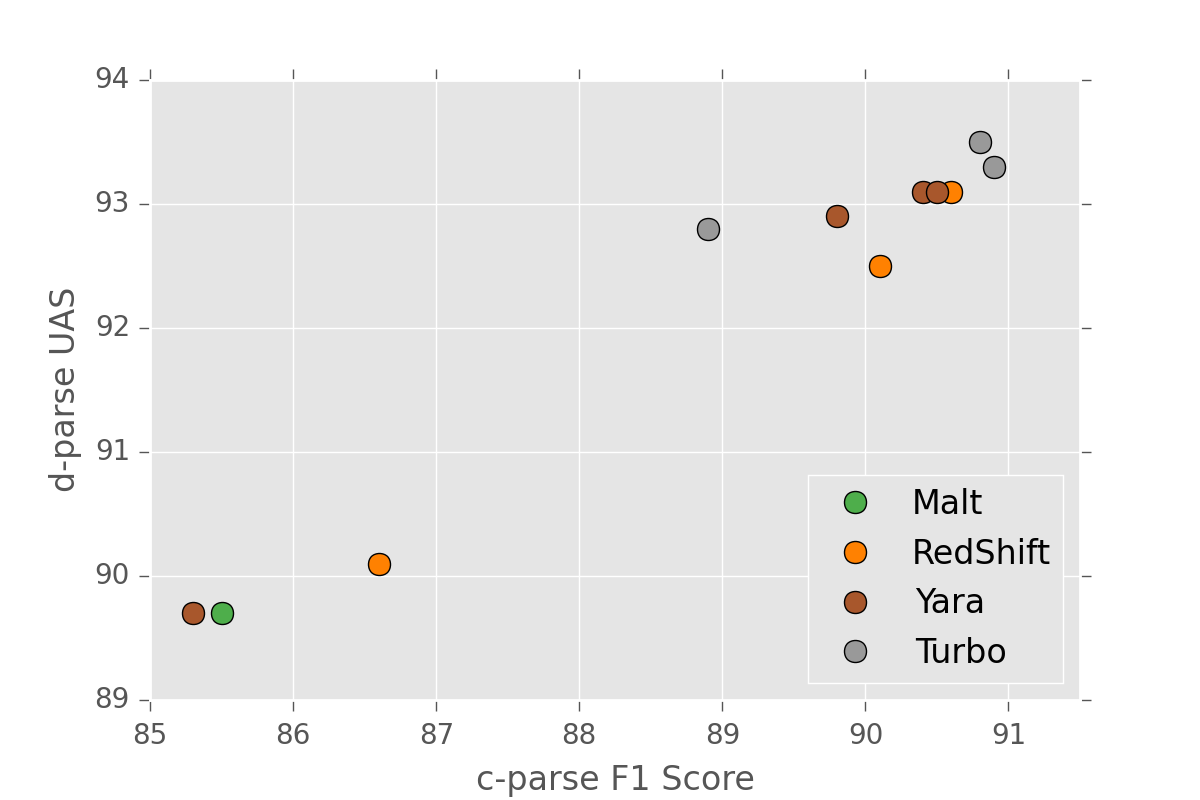
\includegraphics[scale=0.5]{../notebooks/camera_ready_plot.png}
  \begin{tabular}[scale=0.8]{lcccc}
    \toprule
    Model & UAS  & $F_1$ & Sent./s.  & Oracle  \\
    \midrule
    \textsc{MaltParser}  & 89.7 & 85.5 & 240.7& 87.8 \\
    \textsc{RS-K1}       & 90.1 & 86.6 & 233.9& 87.6 \\
    \textsc{RS-K4}       & 92.5 & 90.1 & 151.3& 91.5 \\
    \textsc{RS-K16}      & 93.1 & 90.6 & 58.6 & 92.5 \\
    \textsc{Yara-K1}     & 89.7 & 85.3 & 1265.8 & 86.7 \\
    \textsc{Yara-K16}     & 92.9 & 89.8 & 157.5 & 91.7 \\
    \textsc{Yara-K32}     & 93.1 & 90.4 & 48.3 & 92.0 \\
    \textsc{Yara-K64}     & 93.1 & 90.5 & 47.3 & 92.2 \\
    \textsc{TP-Basic}    & 92.8 & 88.9 & 132.8& 90.8 \\
    \textsc{TP-Standard} & 93.3 & 90.9 & 27.2 & 92.6 \\
    \textsc{TP-Full}     & 93.5 & 90.8 & 13.2 & 92.9 \\
    \bottomrule
  \end{tabular}
  \caption{The effect of d-parsing accuracy (PTB \S 22)
    on \ParseName{} and an oracle converter.  Runtime includes
    d-parsing and c-parsing.  
    Inputs include 
 MaltParser \cite{nivre2006maltparser}, 
    the RedShift implementation of the Zhang-Nivre parser
    \cite{zhang2011transition} with beam size $K \in \{1, 4, 16\}$,
the YaraParser implementation of the Zhang-Nivre parser
    \cite{zhang2011transition} with beam size $K \in \{1, 16, 32, 64\}$, and three versions of TurboParser trained with projective constraints
    \cite{martins2013turning}.
\label{tab:oracle} }

\end{table}


Table~\ref{tab:acc} compares the accuracy and speed of the
phrase-structure trees produced by the parser.  For these experiments
we treat our system and the Zhang-Nivre parser as an independently
trained, but complete end-to-end c-parser. Runtime for these
experiments includes both the time for d-parsing and conversion.
Despite the fixed dependency constraints, the English results show
that the parser is comparable in accuracy to many widely-used systems,
and is significantly faster. The parser most competitive in both speed
and accuracy is that of \newcite{zhu2013fast}, a fast shift-reduce
phrase-structure parser.

Furthermore, the Chinese results suggest that, even without making
language-specific changes in the feature system we can still achieve
competitive parsing accuracy.  
% In future work we hope to add
% additional Chinese specific features to the system.

% explorations like adopting better d-parse systems such as ZPar
% \cite{zhang2011syntactic} and feature engineering a future work.
% (e.g. using the
% last character of a Chinese word as features), Due to the time constraints, 


\paragraph{Effect of Dependencies}

Table~\ref{tab:oracle} shows experiments comparing the effect of
different input d-parses.  For these experiments we used the same
trained parser with seven different d-parsers of varying quality and
speed. We measure for each parser: its UAS, speed, and labeled $F_1$
when used with \ParseName and with an oracle converter.\footnote{For a
  gold parse $y$ and predicted dependencies $\hat{d}$, define the
  oracle parse as $y' = \argmin_{y' \in \mathcal{Y}(x, \hat{d})}
  \Delta(y, y') $} The paired figure shows that there is a direct
correlation between the UAS of the inputs and labeled $F_1$.

% Our next set of experiments look at the effect of different 
% input dependency trees. We ran the same trained converter 
% on seven different dependency inputs of varying quality measured 
% by unlabeled accuracy score (UAS).
% shows the results for each d-parser:  its UAS,
% labeled $F_1$ when it is used with \ParseName and with an oracle converter.\footnote{For a gold parse $y$ and predicted
% dependencies $\hat{d}$, define the oracle parse as
% $y' = \argmin_{y' \in \mathcal{Y}(x, \hat{d})} \Delta(y, y') $}
% Figure~\ref{fig:corr}  shows that there is a direct correlation
% between the UAS of the inputs and labeled $F_1$.
% \nascomment{there was a claim about small changes in d accuracy having
%   big effects, but the plot looks linear to me}
%  , and that small 
% changes in dependency accuracy can have rather large effects.
% For instance MaltParser scores $89.7$ in UAS but the conversion
% produces only a $85.5$ F1 score. 


\begin{figure}
  \centering
  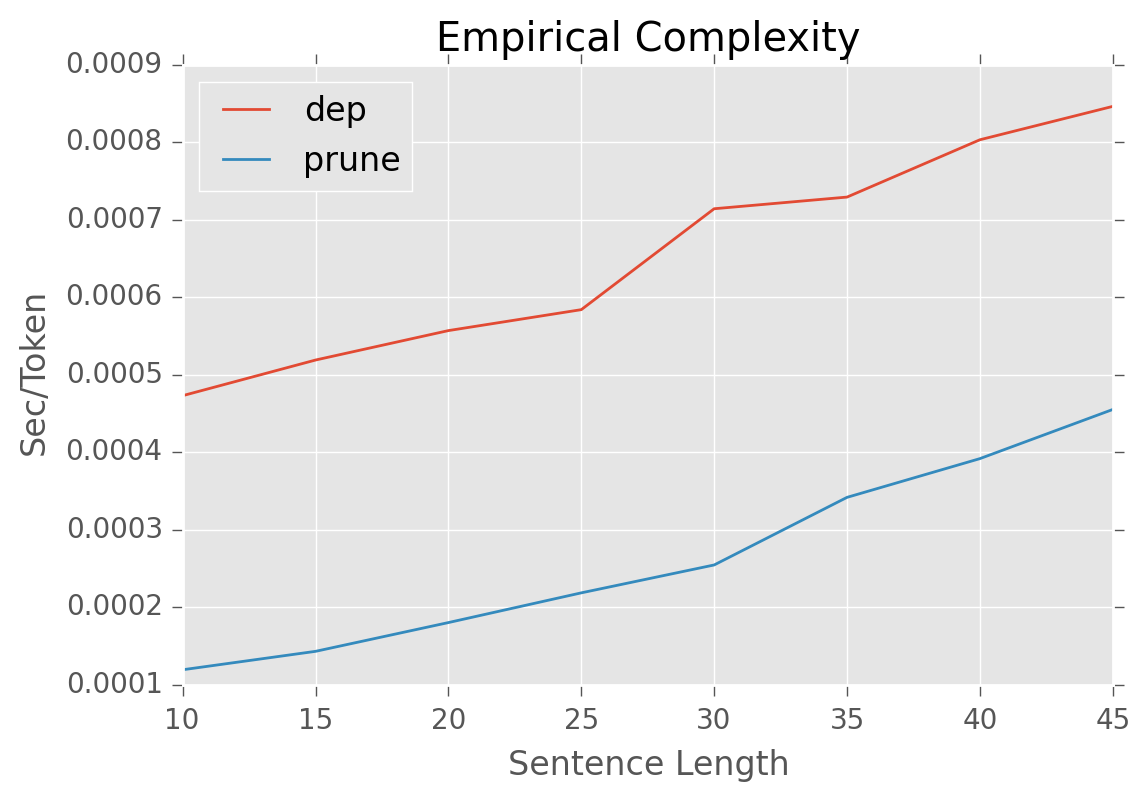
\includegraphics[scale=0.48]{../notebooks/comp}
  \caption{Empirical runtime of the parser on sentences of varying length, with and without pruning. 
  Despite a worst-case quadratic complexity, observed runtime is
  linear.
\label{fig:speed}}
\end{figure}

\paragraph{Runtime}

In Section~\ref{sec:pardeps} we considered the theoretical 
complexity of the parsing model and presented the main 
speed results in Table~\ref{tab:alg-oracle}.
Despite having a quadratic theoretical complexity,
the practical runtime was quite fast.
Here we consider the empirical complexity of the 
model by measuring the time spent on individual sentences. 
Figure~\ref{fig:speed} shows parser speed for
sentences of varying length for both the full algorithm
and  with pruning. In both 
cases the observed runtime is  linear.

\paragraph{Recovering Phrase-Structure Treebanks}
Annotating phrase-structure trees is often more expensive and slower than annotating unlabeled dependency trees \cite{schneider2013framework}. For low-resource languages, an alternative approach to developing fully annotated phrase-structure treebanks might be to label a small amount of c-parses and a large amount of cheaper d-parses. Assuming this setup, we ask how many c-parses would be necessary to obtain reasonable performance?

For this experiment, we train \ParseName on only 5\% of the PTB training set and apply it to predicted d-parses from a fully-trained model. Even with this small amount of 
data, we obtain a parser with development score of  $F_1 = 89.1\%$, which is comparable to \newcite{charniak2000maximum} and Stanford PCFG \cite{klein2003accurate} trained on the complete c-parse training set. Additionally, if the gold dependencies are available, \ParseName{} with 5\% training achieves $F_1 = 95.8\%$ on development, demonstrating a strong ablity to recover the phrase-structure trees from dependency annotations.


% Our next set of experiments consider the efficiency of the model. For these experiments we consider both the full and pruned version of the parser using the pruning described in section~\ref{sec:prune}. Table~\ref{tab:speed} shows that in practice the parser is quite fast,  averaging around \% tokens per second at high accuracy.

% We also consider the end-to-end speed of the parser when combined with different downstream dependencies. We look at

% Finally we consider the empirical run-time of the parser on sentences of different length. Figure~\ref{fig:speed} shows the graph.






\begin{table}
  \centering
  \footnotesize
  \begin{tabular}{ccccc}
    \toprule
    \multicolumn{3}{c}{Class} & \multicolumn{2}{c}{Results} \\
    Dep. & Span & Split & Count & Acc.  \\ 
    $(h, m)$ & $\Span{i,j}$ & $k$ &  & $A$ \\ 
    \midrule
    + & + & +  &  32853 &  97.9   \\ 
    -- & + & +  &  381 & 69.3   \\ 
    + & + & --  &  802   & 83.3   \\ 
    -- & + & --  &  496 & 85.9   \\ 
    + & -- & --  &  1717 & 0.0    \\ 
    -- & -- & --  &  1794 & 0.0    \\ 
    \bottomrule
  \end{tabular}
  \caption{Error analysis of binary CFG rules. Rules used are split into classes based on 
    correct (+) identification of dependency $(h,m)$, span $\Span{i,j}$, and split $k$. 
    ``Count'' is the size of each class. ``Acc.'' is the accuracy of span nonterminal identification. \label{tab:analysis}}
\end{table}

% \paragraph{Conversion}

% Previous work on this problem has looked at converting dependency trees to phrase-structure trees using linguistic rules \cite{xia2001converting,xia2009towards}. This work is targeted towards the development of treebanks, particularly converting dependency treebanks to phrase-structure treebanks.
% For this application, it is useful to convert gold trees as opposed to predicted trees.




% To compare to this work, we train our parser with gold tags and run on gold dependency trees in development. Table~\ref{tab:convert} give the results for this task.

% \paragraph{Conversion for Training}


% \lpkcomment{quick highlights... need rewrite}
% Annotating unlabeled dependency has been proven to be cheaper and faster than annotating phrase structure. \cite{nathanandhisfriends}
% What if we need the phrase-structure trees? Our parser given a chance to annotate more dependencies, while get a good phrase-structure parser.

% Show in Figure \ref{fig:dataamo}. We train a simple PCFG model with $vMarkov =2$ and $hMarkov = 2$ \cite{parentannotate}.

% The are two scenarios here, blue and red.

% Blue means we label whole phrase-structure parse tree, given 5\%, 20\%, 50\%, 80\% and 100\% annotation of the PTB, the parser's performance goes up, but this way is expensive.

% Red means we only label 5\% phrase-structure parses, and then we train our parser on this 5\% phrase-structure model (with dependencies extracted using collins headrule), then, we use our parser's predicted phrase-structure tree (predicted on gold dependency parses, assuming people are annotating that), from 20\% to 100\%, to train the phrase-structure parser.

% We note that the accuracy of the PCFG model also goes higher with more dependency annotations, which suggests a cheaper and fast (?) way to build a language resource in phrase-structure.

% \begin{figure}
%   \centering
%   % \begin{tabular}{|l|ll|}
%   %   \hline
%   %   Model & fscore & speed  \\
%   %   \hline
%   %   \textsc{TurboParser} & & \\
%   %   \textsc{MaltParser} & & \\
%   %   \textsc{MIT} & & \\
%   %   \hline
%   % \end{tabular}


%   \label{tab:speed}
%   \caption{Experiments of parsing speed. (a) The speed of the parser on its own and with pruning. (b) The end-to-end speed of the parser when combined with different dependency parsers. }
% \end{figure}

\paragraph{Analysis}
\label{sec:analysis}
Finally we consider an internal error analysis of
the parser. For this analysis, we group each binary rule production
selected by the parser by three properties:
Is its dependency $(h, m)$ correct? Is its span $\Span{i,j}$ correct? 
Is its split $k$ correct? The first property is fully determined by the 
input d-parse, the others are partially determined by \ParseName itself.

Table~\ref{tab:analysis} shows the breakdown. The
conversion is almost always accurate ($\sim$98\%) when the parser has correct span and
dependency information. As expected, the difficult cases come when the dependency
was fully incorrect, or there is a propagated span mistake. As dependency parsers
improve, the performance of \ParseName{} should improve as well.
 


% \begin{itemize}
% \item Dep
% \item Span
% \item Split
% \end{itemize}

% We also consider the mistakes that are made by the parser compared to the
% mistakes made. For each of the bracketing errors made by the parser, we can classify it as a bracketing mistake, a dependency mistake or neither.



% \begin{figure}
%   \centering
%   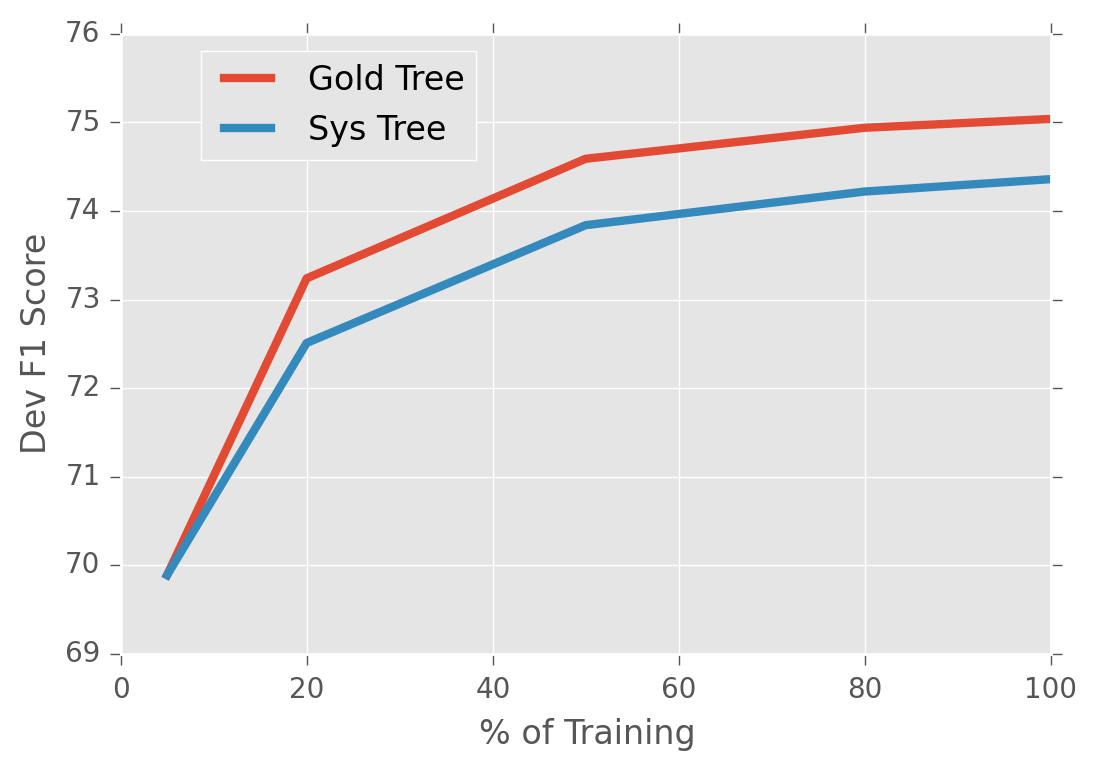
\includegraphics[scale=0.4]{../notebooks/data}
% \label{fig:dataamo}
% \end{figure}

% \nascomment{missing:  the part about varying the amount of labeled
%   constituent data}



\section{Conclusion}

With recent advances in statistical dependency parsing, we find that
fast, high-quality phrase-structure parsing is achievable using dependency
parsing first, followed by a statistical conversion algorithm to
fill in phrase-structure trees. 
Our implementation is available as open-source software at \ParserUrl.

\section*{Acknowledgments}
% NSF PARTIAL project
The authors thank the anonymous reviewers
and Andr\'{e} Martins, Chris Dyer, and Slav Petrov \nascomment{who to thank?  Andr\'{e}?  cite their tech report
  somewhere?  who else?} for helpful feedback.
This research was supported in part by NSF grant IIS-1352440 and computing resources provided by Google and the Pittsburgh Supercomputing Center.


% One question for future work is whether these results are language
% dependent, or whether these transformation can be projected across
% languages. If this were possible, we could use a system of this form to learn phrase
% structure parsers on languages with only dependency annotations.





% \appendix{}

% \section{Proof of PS Size}
% \label{app:proof}

% Consider the LCFG grammar with two rules $A = \RuleA{X}{X}{X}$ and  $ B = \RuleB{X}{X}{X}$ and a sentence $x_1, \ldots, x_{2n+1}$. Let the dependency parse be defined as $d_{n+1} = 0$ and $d_i = n+1$ for all $i \neq n + 1$, i.e.

% \begin{center}

% \scalebox{0.5}{
% \begin{dependency}[theme=simple]
%   \begin{deptext}[column sep=0.7cm]
%     $1$ \& $2$ \& \ldots \& $n+1$ \& $\ldots$ \& $2n$ \& $2n+1$ \\
%   \end{deptext}
%   \deproot{4}{ROOT}
%   \depedge{4}{1}{}
%   \depedge{4}{2}{}
%   \depedge{4}{6}{}
%   \depedge{4}{7}{}
% \end{dependency}
% }
% \end{center}

% \noindent Since all rules have $h = x_n$ as head, a parse is a chain of $2n$ rules with each rule in $\{A, B\}$, e.g. the following are $BB...$, $BA...$, $AA...$

% \begin{center}

% \scalebox{0.6} {
% \Tree [ .X $x_1$ [ .X $x_2$  [ .$\vdots$ $x_{n+1}$ ]   ] ]
% \Tree [ .X $x_1$ [ .X  [ .$\vdots$ $x_{n+1}$ ] $x_{2n+1}$  ] ]
% \Tree [ .X  [ .X  [ .$\vdots$ $x_{n+1}$ ]   $x_{2n}$ ] $x_{2n+1}$ ]
% }
% \end{center}


% \noindent Since there must be equal $A$s and $B$s and all orders are possible, there are $2n \choose n$ valid parses and $|\mathcal{Y}(x, d)|$ is $O(2^n)$.
% \textbf{Acknowledgment} sections should go as a last (unnumbered) section immediately
% before the references.



\bibliography{full}
\bibliographystyle{naaclhlt2015}

\end{document}

%%% Local Variables:
%%% mode: latex
%%% TeX-master: t
%%% End
